\chapter{Risultati e Analisi}
\label{cha:risultati}
\section{Confronto veicolo Ego Simulato e veicolo Leader}
In questa sezione verranno analizzati i risultati della simulazione del veicolo \emph{ego} confrontandoli 
con i dati del veicolo \emph{leader}. L'obiettivo è valutare l'accuratezza e l'efficacia del modello di guida autonomo nel replicare 
il comportamento del veicolo che lo precede.
\subsection{Accelerazione}
In Figura \ref{fig:acc_leader_ego} viene presentato un confronto tra l'accelerazione del veicolo \emph{leader} 
(linea arancione) e quella del veicolo \emph{ego} simulato (linea blu).
\begin{figure}[H]
    \centering
    \adjustbox{center}{
        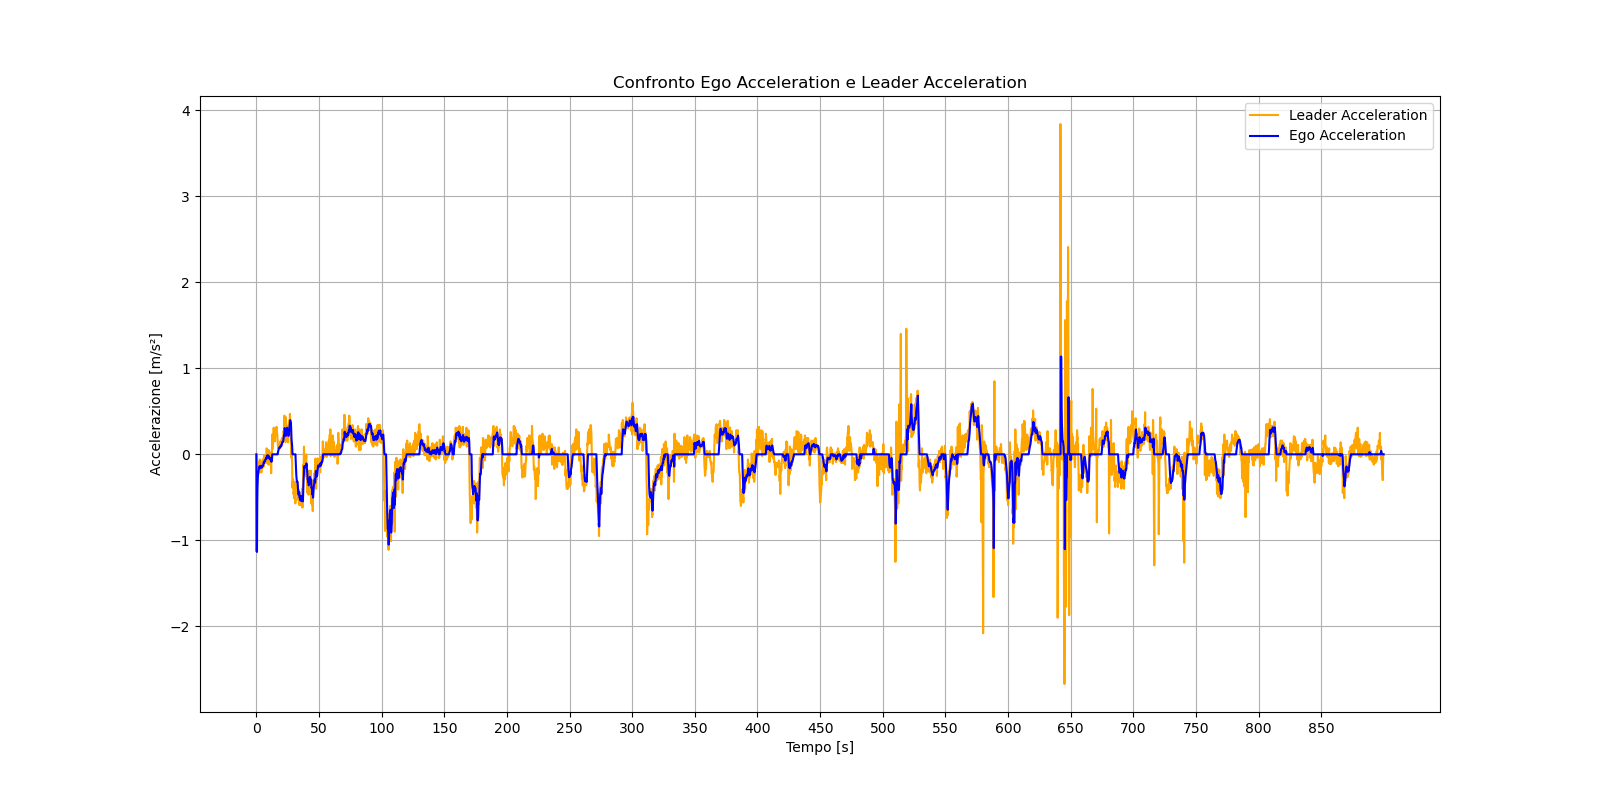
\includegraphics[width=1.25\linewidth]{simulation/leader_comparison/acceleration.png}
    }
    \caption{Confronto tra ego\_acceleration simulata e leader\_acceleration}
    \label{fig:acc_leader_ego}
\end{figure}
\noindent Si osserva che il veicolo \emph{ego} simulato segue in modo coerente l'accelerazione del veicolo \emph{leader}. Tuttavia, la 
risposta del veicolo \emph{ego} risulta significativamente più smussata, priva dei rapidi picchi e delle fluttuazioni ad alta frequenza 
presenti nel segnale del \emph{leader}. Questo indica che il modello di simulazione applica correttamente filtraggio e smorzamento, 
contribuendo a una guida più stabile e confortevole, riducendo l'impatto di variazioni brusche.
\\\\
\noindent In particolare, intorno ai 650 secondi, il veicolo \emph{leader} presenta un'accelerazione molto elevata seguita da una decelerazione 
altrettanto intensa. Il veicolo \emph{ego} reagisce a questo evento, ma in modo significativamente più moderato, con picchi di accelerazione 
e decelerazione di entità decisamente inferiore.
\\\\
\noindent Per validare ulteriormente il risultato ottenuto, è stato applicato lo stesso filtro passa basso all'accelerazione del veicolo 
\emph{leader} e successivamente è stato calcolato il coefficiente di correlazione di \textbf{Pearson} tra le due curve. Il test ha restituito un 
valore di 0.792, confermando una buona similitudine tra il trend filtrato del leader e l'accelerazione simulata dell'ego.
\\\\
\noindent In conclusione, il grafico mostra che, pur non replicando ogni singola fluttuazione del veicolo \emph{leader}, 
il veicolo \emph{ego} segue fedelmente il trend generale. Il sistema di controllo si dimostra efficace nel garantire 
una dinamica di guida sicura e prevedibile, attenuando le variazioni più estreme dell'accelerazione e favorendo 
un comportamento più lineare e controllato.

\subsection{Velocità}
Il grafico in Figura \ref{fig:vel_leader_ego} mostra il confronto tra la velocità del veicolo \emph{leader} 
(linea arancione) e quella del veicolo \emph{ego} simulato (linea blu).
\begin{figure}[H]
    \centering
    \adjustbox{center}{
        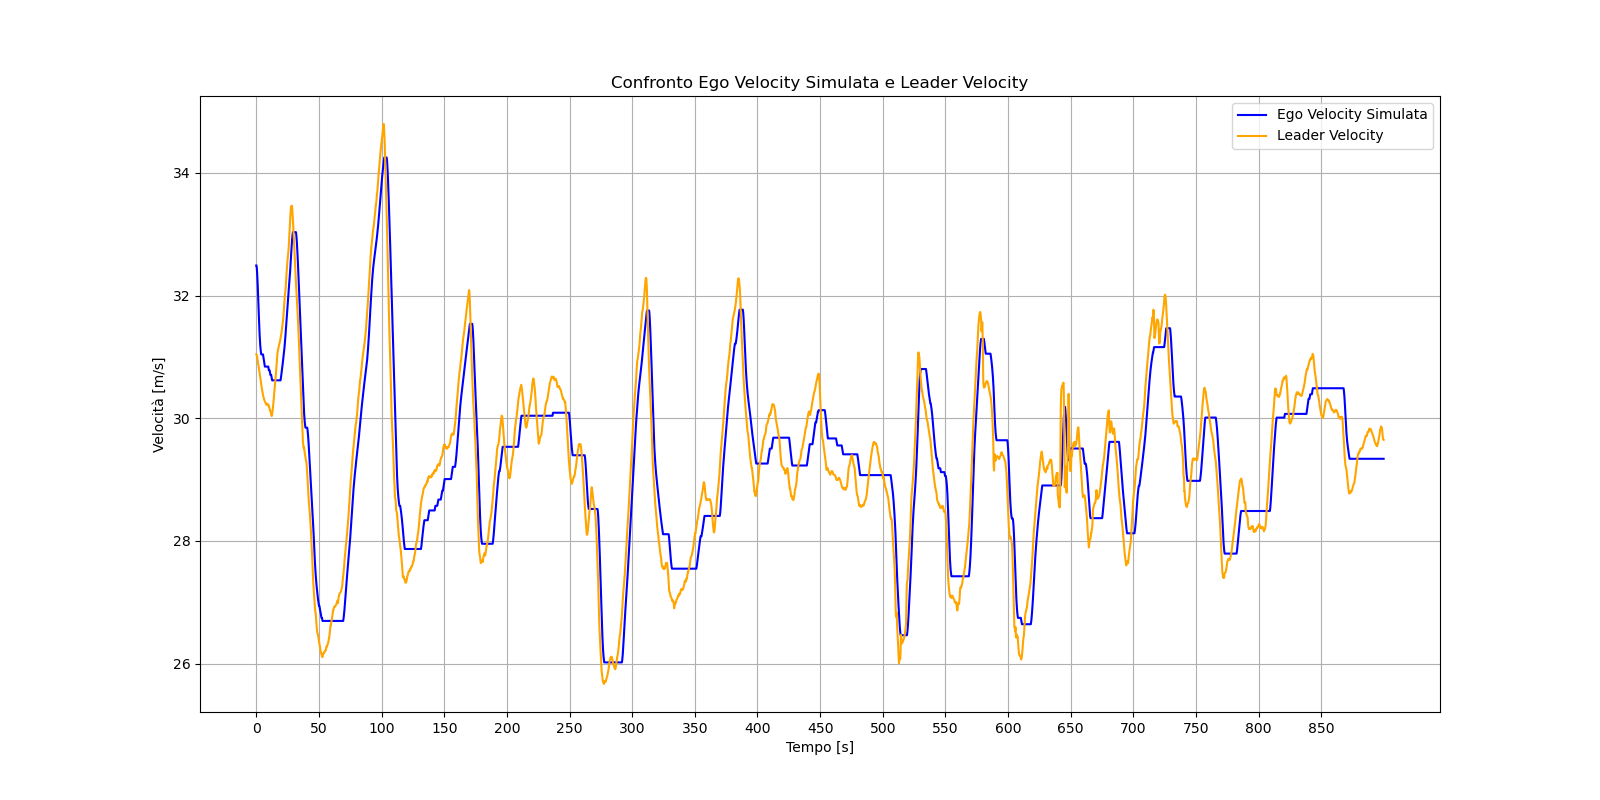
\includegraphics[width=1.25\linewidth]{simulation/leader_comparison/velocity.png}
    }
    \caption{Confronto tra ego\_velocity simulata e leader\_velocity}
    \label{fig:vel_leader_ego}
\end{figure}
\noindent A differenza del grafico dell'accelerazione, dove il segnale del veicolo \emph{ego} appariva smussato, il grafico della 
velocità mostra una notevole sovrapposizione tra i due profili. Questo indica che il veicolo \emph{ego} è in grado di replicare l
a velocità del veicolo \emph{leader} con elevata precisione, seguendo fedelmente sia le fasi di accelerazione che quele di decelerazione.
\\\\
\noindent Le piccole discrepanze tra le due curve, osservabili in alcuni punti, non compromettono la robustezza complessiva del modello. 
Queste leggere variazioni sono la conseguenza della risposta smorzata dell'accelerazione, che, come visto in precedenza, 
limita reazioni brusche. Nonostante tali attenuazioni, il veicolo \emph{ego} mantiene una velocità che rispecchia fedelmente 
il comportamento del veicolo \emph{leader}.
\\\\
\noindent Anche in questo caso, per validare ulteriormente il risultato ottenuto, è stato calcolato il coefficiente di correlazione 
di \textbf{Pearson} tra le due curve. Il test ha restituito un valore di 0.923, confermando l'elevata similitudine tra la 
velocità simulata dell'\emph{ego} e quella del \emph{leader}.
\\\\
\noindent In conclusione, la simulazione conferma l'elevata efficacia del sistema di controllo della velocità. Il veicolo \emph{ego}
è in grado di mantenere una velocità allineata a quella del \emph{leader}, garantendo una guida fluida e sicura, 
e dimostrando che le attenuazioni nella risposta dell'accelerazione non compromettono la capacità di seguire il profilo di velocità 
desiderato.